%------------------------------------------------
\section{Легкие частицы}

\begin{frame}
	\frametitle{Особенности ускорения легких частиц}
\par В классической регулярной структуре критическая энергия приблизительно равна бетатронной частице $\gamma_{\text{tr}}\simeq\nu_{\text{s}}$ и не зависит от типа частиц.
\newline
\par При одинаковой магнитной жесткости максимальная энергия для легких частиц больше, чем для тяжелых ионов, из-за их отношения заряда к массе. Это означает, что тяжелоионная структура, оптимизированная для работы с определенной критической энергией, потребует преодоления при работе с легкими частицами.
\end{frame}

%------------------------------------------------
\begin{frame}
	\frametitle{Критическая энергия}
     	Коэффициент уплотнения орбиты (momentum compaction factor)
     \small \begin{equation}
     	\alpha=\frac{1}{{\gamma_{\textrm{tr}}}^2}=\frac{1}{C}\int_{0}^{C}{\frac{D\left(s\right)}{\rho\left(s\right)}ds}
     \end{equation} \normalsize 	
     	Частота продольных колебаний пропорциональна коэффиценту проскальзывания (slip-factor)
	\begin{equation}
		 \omega_s\ \sim \eta, \quad \eta=\eta_0=1/\gamma_{tr}^2-1/\gamma^2
	 \end{equation} \normalsize 	
	При приближении энергии критической нарушается адиабатичность продольного фазового движения, а также значительное воздействие нелинейного эффекта более высоких порядков разброса импульса
	 
\end{frame}

%------------------------------------------------
\begin{frame}
	\frametitle{Суперпериодическая модуляция}
     Уравнение дисперсионной функции с бипериодической фокусировкой
         \small \begin{equation}
	   \frac{d^2D}{ds^2}+\left[K(s)+\varepsilon k(s)\right]D=\frac{1}{\rho(s)}
	 \end{equation} \normalsize 	
\small \begin{equation}
\alpha_{\text{s}}=\frac{1}{\nu^2_{x, \text {arc}}}\left\{1+\frac{1}{4}\left(\frac{\bar{R}_{\text {arc}}}{\nu_{x, \text {arc}}}\right)^4 \sum_{k=-\infty}^{\infty} \frac{g^2_k}{\left(1-k S / \nu_{x, \text {arc}}\right)\left[1-\left(1-k S / \nu_{x, \text {arc}}\right)^2\right]^2} \cdots\right\}
\end{equation} \normalsize 	
	\begin{figure}[h!]
		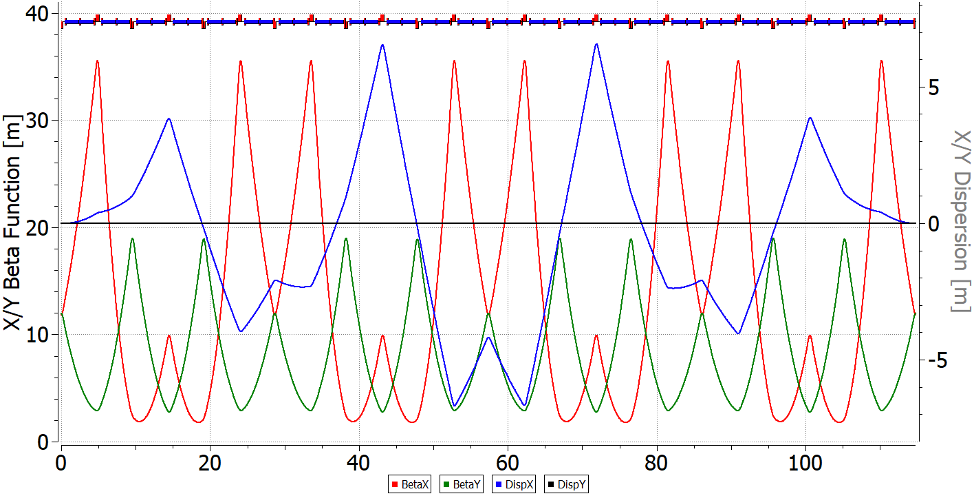
\includegraphics[width=6.5cm]{images/resonant_arc}
		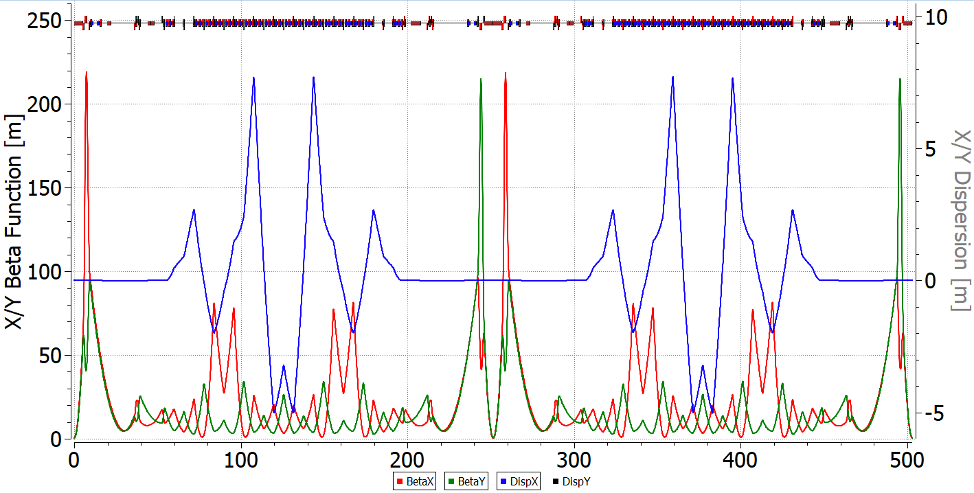
\includegraphics[angle=0, width=6.5cm]{resonant}
                \label{Figure 1}
	\end{figure}
	
	                
	

	 
\end{frame}